\documentclass[conference,compsoc]{IEEEtran}
\usepackage[utf8]{inputenc}
\usepackage{cite}
\usepackage{graphicx}
\usepackage{multirow}
\usepackage{float}
\graphicspath{ {./images/} }

\usepackage[hyphens]{url}
\usepackage[hidelinks]{hyperref}
\hypersetup{breaklinks=true}

\usepackage{caption}
\captionsetup[table]{skip=10pt}


\begin{document}

\title{A Survey on Smartphone Ad Hoc Networks}

\author{\IEEEauthorblockN{Matouš Skála}
\IEEEauthorblockA{Delft University of Technology\\
Email: M.Skala@student.tudelft.nl}}

\maketitle

\begin{abstract}

In this survey, we explore different nearby communication technologies  present in today's smartphones and discuss their implementation within Android OS. We explain challenges of deploying a large-scale smartphone ad hoc network and analyze available state-of-the-art applications and SDKs for nearby device communication. Finally, we design a proof of concept application for Android to demonstrate the feasibility of mesh networking within the constraints imposed by the operating system.

\end{abstract}

\begin{IEEEkeywords}mesh networks, mobile ad hoc networks\end{IEEEkeywords}

\section{Introduction}

There has been a desire to provide a reliable omni-present communication protocol since the beginning of the Internet. To this day, more than half the world's population is interconnected. However, the growth has slown down and there are still rural areas where reliable Internet connection is not available. The industry has tried to tackle reachability issues with initiatives such as Google's Project Loon\footnote{\url{https://loon.com/}} or Facebook's internet.org\footnote{\url{https://internet.org/}}. At the same time, numerous self-organized communities around the world are establishing \textit{wireless community networks}, providing an alternative to traditional Internet service providers. \cite{wcn}


On the other hand, there are countries where the communication is restricted or censored, preventing people from communicating freely. Moreover, even in places with relatively mature infrastructure, there are occasionally connectivity issues at places with high gatherings of people, such as conferences or festivals, causing congestion in the infrastructure networks.

The increasing capabilities of smartphones and novel wireless networking technologies open up possibilities to a whole new range of applications that can communicate without the need for the Internet connection. Prospective use cases are ranging from proximity-based social networks, infrastructure-less communication with \textit{Internet of Things (IoT)} devices, student attendance tracking, to communication between attendees during music festivals or protests, where the cellular network is overloaded or censored. The practical usability of the mesh networking technology has been demonstrated during the Hong Kong protests in 2018 and 2019, where protesters relied on peer-to-peer communicaion apps as a communication tactic. \cite{forbes:hk}

% beginning of internet, decentralization
% people without connectivity, rural areas
% congestion - conferences, festivals
% mesh networking - contrast in topology, no centralized entity eliminates single point of failure, self healing
% dates back to 50s - military, academic, governmental use cases
% today's devices
% hybrid networks - last mile connectivity



This survey is structured as follows. In Section \ref{wirelesstech}, we first analyze capabilities of various wireless communication technologies and their implementation and possible limitations within Android OS. In Section \ref{routing}, we discuss the problem of routing in mobile ad hoc networks and list commonly used routing algorithms.
In Section \ref{applications}, we explore different Android applications taking advantage of mesh networking for censorship resilient messaging. In Section \ref{poc} we present our proof of concept for deploying an ad hoc network with multi-hop routing on Android. Finally, Section \ref{conclusion} concludes this work.

\section{Wireless Communication Technologies} \label{wirelesstech}

Over the past few years, smartphones have become powerful devices that come equipped with numerous network connectivity modules. In addition to \textit{Bluetooth} and \textit{Bluetooth Low Energy} (BLE) \cite{android:ble}, most recent devices also come with support for \textit{Wi-Fi Direct} \cite{android:wifip2p} and \textit{Wi-Fi Aware} \cite{android:wifiaware}.
% to facilitate the interconnection with nearby devices over longer distances and with higher bandwidth.

Wi-Fi Direct, also referred to as \textit{Wi-Fi peer-to-peer}, allows device-to-device Wi-Fi communication without an additional \textit{access point (AP)}. From Android 8.0, the Wi-Fi Aware  standard, also known as \textit{Neighbor Awareness Networking (NAN)}, has been supported, allowing to automatically form clusters of nearby devices.

Wi-Fi generally offers a higher range of coverage and bandwidth than Bluetooth, so it might be more suitable for data-intensive applications such as photo or video sharing. On the other hand, Bluetooth is supported on a wider variety of devices and especially BLE can result in significantly lower battery consumption, thus it is more suitable for transferring small amounts of data such as text messages.

In Table \ref{wirelesstech_table}, we can find an overview of all communication technologies supported by Android OS that are described in this section. For each technology, there is a version of Android from which it is officially supported, as well as a theoretical throughput and range specified by its respective specification.

\begin{table}
  \centering
  \begin{tabular}{ | l | l | l | l | l | }
    \hline
    Technology & Android & Throughput & Range \\
    \hline
    Bluetooth & 2.0+ & 2 Mbps & $\sim$40 m \\
    \hline
    BLE Advertising & 4.3+ & \multirow{3}{*}{0.3 Mbps} & \multirow{3}{*}{$\sim$100 m} \\
    BLE GATT & 5.0+ &  &  \\
    BLE L2CAP & 10.0+ &  &  \\
    \hline
    Wi-Fi Direct & 4.0+ & \multirow{2}{*}{250 Mbps} & \multirow{2}{*}{$\sim$200 m} \\
    Wi-Fi Aware & 8.0+ & & \\
    \hline
  \end{tabular}
  \caption{Comparison of wireless communication technologies supported by Android OS %w.r.t. supported Android platform versions, a theoretical throughput, and range
  }
  \label{wirelesstech_table}
\end{table}


\subsection{Bluetooth}\label{bluetooth}
Bluetooth is a wireless data exchange standard developed by Bluetooth SIG and supported by the majority of mobile devices. To connect two devices, one device
 (a \textit{server}) first needs to make itself discoverable. On Android, the application can request device discoverability for a specified duration, but this action needs to be confirmed by the user in a dialog presented by the system. Then, other devices (\textit{clients}) can start scanning to find MAC addresses of nearby Bluetooth devices.

\subsubsection{Radio Frequency Communication (RFCOMM)}
It is possible to establish a channel between two devices using the \textit{RFCOMM} protocol. First, the server opens a server socket. Clients can then use the discovered MAC address to initiate the connection with the server. This method allows to open a secure channel either between two \textit{paired} devices, or even an insecure one without need of going through the pairing process.

When two devices are linked, one of them takes the role of a \textit{master}, the other one is a \textit{slave}. There can be up to 7 slaves connected to a single master and such a network is called a \textit{piconet}. A device can only be a master of a single piconet. However, since Bluetooth 4.1, it is possible for a slave to connect to multiple masters, or for a master to also act as a slave in another piconet. A network consisting of multiple piconects is referred to as a \textit{scatternet}. \cite{bluetooth51spec}

\subsection{Bluetooth Low Energy}
BLE was first introduced in the Bluetooth 4.0 specification as a power-efficient way to connect with peripherals to exchange small amounts of data. It offers a similar range as Bluetooth with a lower throughput, but a significantly lower power consumption in an idle state. That makes it suitable for sending short bursts of data.

Like Bluetooth, BLE operates in the 2.4 GHz radio band. There are 40 physical channels, 3 of them are used for advertising and 37 are used as data channels. Devices that transmit unidirectional broadcasts on advertising channels are called \textit{advertisers}. Devices that receive data on advertising channels are called \textit{scanners}. Advertisement transmission occurs in advertising events. At the beginning of each event, the advertiser sends an advertising packet. Upon detection of the advertisement, the scanner may send a \textit{scan request}, which is then followed by a \textit{scan response} from the advertiser. The advertisement packet can be sent in all 3 advertising channels during the same advertising event. Both advertisement and scan response size are limited to 31 bytes, but can be extended up to 255 bytes by using extended advertisements in Bluetooth 5.0. \cite{bluetooth51spec}

If the advertising event is marked as connectable, the advertiser may receive connection requests from other devices referred to as \textit{initiators}.

\subsubsection{Generic Attribute Profile (GATT)}
%BLE devices can act in two roles: \textit{centrals} and \textit{peripherals}. The peripheral device starts by broadcasting an advertising packet limited to the size of 31 bytes. Central devices can then run a scanning process and filter advertising packets based on the MAC address, service UUID, or other parameters.
BLE devices usually communicate using the \textit{Generic Attribute Profile} (GATT). There are two roles in GATT: a \textit{server} and a \textit{client}.
%Both central and peripheral can act as a server or client.
The GATT server allows to store short pieces of data known as \textit{attributes} in form of \textit{characteristics} and their \textit{descriptors}. Once a client establishes a connection with a server, it can send requests to \textit{read} or \textit{write} supported attributes. The server can also actively push messages to clients using \textit{notify} and and \textit{indicate} operations. The difference is that notifications are unacknowledged, while indications require acknowledgments. They are usually used to notify clients that a value of characteristics has changed.

\subsubsection{Logical Link Control and Adaptation Layer Protocol (L2CAP)}
From Android 10, there is also a possibility to form a connection-oriented \textit{L2CAP} channel between BLE devices, which enables direct access to Bluetooth sockets.

\subsubsection{Discovery using BLE}

As mentioned in \ref{bluetooth}, connecting to a Bluetooth device usually involves a discovery mechanism to obtain the MAC address of the target device. This requires the user to make the device discoverable. To establish Bluetooth connections without user interaction, BLE can be used to transfer MAC address using BLE advertising packets.

It is important to note that due to \textit{Bluetooth LE Privacy} \cite{ble:privacy}, the MAC address received in advertising packets is randomly generated if the devices are not paired. Therefore, it cannot be used to create a Bluetooth socket. However, the advertising packet can be abused to include the physical MAC address as part of the service UUID. Once the receiver extracts the physical MAC address from the packet, it can connect to the Bluetooth socket of the server. This is probably the most accessible way to create Bluetooth sockets between two devices without any user interaction. \cite{btautoconnect}

Unfortunately, starting with Android 8, it is no longer possible to obtain a local MAC address programatically, so this solution would now require the user to manually enter the device MAC address from the system settings.

\subsection{Wi-Fi Direct}

There have been many attempts to enable direct communication between IEEE 802.11 radio devices. The 802.11 standard defines two operating modes. Next to the traditional \textit{infrastructure} mode, there is an \textit{ad-hoc} mode which allows device-to-device communication. However, the ad-hoc mode is not supported by Android OS, even though it can be enabled on some devices with a root access.

\textit{Wi-Fi Direct} (also known as Wi-Fi Peer-to-Peer) \cite{wifip2p} is a IEEE 802.11 based protocol released by Wi-FI Alliance in 2009 and supported from Android 4.0. With Wi-Fi direct, devices are organized in groups, where one device is the Group Owner (GO) and the rest are Group Members (GM). The roles are not predefined, but are negotiated during the group formation process. Groups are able to support Legacy Clients (LC), which means that even devices without Wi-Fi Direct support can join as group members.

\subsubsection{Multi-group communication}

The standard only defines intra-group communication, but it does not restrict a Group Member from participating in multiple groups simultaneously. Moreover, a device can theoretically connect both to Wi-Fi Direct and an infrastructure network by using multiple virtual MAC entities. However, these functionalities are not defined by the standard and thus depend on the implementation.
%\subsubsection{Limitations of Android}
In Android, the GO always has the same hardcoded IP address (192.168.49.1), while GM are assigned a random address from the same subnet (192.168.49.2-254). As a result, the scenario where the device would act in multiple groups at the same time cannot be directly implemented.

There are several workarounds proposed in \cite{FunaiTH16}. The first solution is to use \textit{time sharing} to allow a device to act as a gateway between multiple groups. It requires a device to periodically disconnect and reconnect to different groups and effectively act as a relay passing messages between multiple groups.
Another solution takes advantage of \textit{simultaneous connections} using Wi-Fi Direct and the traditional Wi-Fi. The GO advertises its group using a unique Service Set ID (SSID) that can be used by other clients not supporting the framework to join the group. Experiments have shown that it is possible to create a LC/GM gateway node when communicating using multicast UDP datagram sockets. Due to routing-related issues, this solution does not work with traditional datagram or stream sockets. The authors also propose a more efficient \textit{hybrid} protocol that uses multicast sockets as a control channel that triggers gateway configuration change if needed. However, all solutions rely on undocumented behaviors, which means their reliability can vary across devices or Android OS versions.

\subsection{Wi-Fi Aware}

\textit{Wi-Fi Aware}, also known as \textit{Neighbor Awareness Networking} (NAN) is a recent networking standard introduced by Wi-Fi Alliance. \cite{wifiaware} It works by forming clusters with nearby devices. The discovery process starts when one device (a \textit{publisher}) publishes a discoverable service. Other devices (\textit{subscribers}) who subscribe to the same service will receive a notification once a matching publisher is discovered. After the subscriber discovers a publisher, it can either send a short message or establish a network connection with the device. A device can be both a subscriber and a publisher simultaneously.


\subsubsection{Ranging peers}

Devices that are equipped with \textit{Wi-Fi Round Trip Time} (RTT) can also directly measure distance to peers. This information can further be used for location-aware service discovery. Specifically, the discovery process can be restricted to only include services within a particular range specified by a minimum and maximum distance in meters.

\subsubsection{Wi-Fi Aware on Android}

Wi-Fi Aware is supported by Android OS since the version 8.0. However, it is not required by Google for devices to support this standard. During our testing, it was available only on a small subset of potentially capable devices. For example, Google Pixel and Samsung Galaxy S9 do not support Wi-Fi Aware, while they officially support Android later than 8.0. In fact, Google Pixel 2 XL and 4 XL were the only supported devices we were able to test. This makes it impractical to use it as the only communication protocol even for new apps.

To our best knowledge, there have been no attempts to utilize Wi-Fi Aware as a communication layer for mesh networks so far. It has a higher throughput and range then Bluetooth. It also should not suffer from the issues related to Wi-Fi Direct described previously. However, reluctant support from device manufacturers prevents it from being useful for a wide-scale deployment in the near future.


\section{Routing Protocols}\label{routing}


%// motivation for routing in manets, issues, topology changes

There are several approaches for disseminating content in ad hoc networks. In general, we can divide protocols into two main categories: flooding-based and routing-based.

Flooding-based solutions do not perform routing, instead packets are broadcasted by nodes and spread across the whole network. In naive flooding, \textit{broadcast storms} can happen in case nodes broadcast the same packet repeatedly. Therefore, nodes should implement loop prevention by storing a set of recently received messages and only deliver messages that have not been received before. \cite{flooding} While conceptually simple, flooding incurs high overhead in terms of transmitted messages, especially when only point-to-point communication between two devices is desired.

Routing-based protocols can be classified into tree types: \textit{proactive} (table-driven), \textit{reactive} (on-demand), and \textit{hybrid}.

\subsection{Proactive}

In proactive routing protocols, each node maintains routes to every other node in the network. The routes information is usually stored in routing tables and it is periodically updated as the topology changes. \cite{routing} Examples of proactive routing protocols are Destination Sequence Distance Vector (DSDV) \cite{dsdv} or Optimized Link State Routing (OLSR) \cite{olsr}.

\subsection{Reactive}

In reactive routing, routes are established on demand. When a node needs to send a message to the destination and the route is not known, the \textit{route discovery} mechanism is invoked. This is usually done by broadcasting a route discovery packet through the network. Once the path between the source and the destination is known, data can be transmitted using the selected route. Due to dynamic nature of SPANs, a \textit{route maintenance} mechanism is required to handle route breakage.
Some well-known reactive routing protocols are Ad Hoc On-Demand Distance Vector (AODV) \cite{aodv} or Dynamic Source Routing (DSR) \cite{dsr}.

%Compared to proactive approach, this is more efficient in larger networks, as the whole topology does not have to be synchronized. However, it incurrs a time delay before the first message to the destionation can be sent.

%Hybrid protocols allow to combine both approaches. \cite{routing}


%\subsection{Hybrid}

%\section{Implementation in Android OS} \label{android}
%\subsection{BluetoothManager}
%\subsection{WifiP2pManager}
%\subsection{WifiAwareManager}
%\subsection{Nearby Connections API}


\section{Mesh Networking Applications \& SDKs} \label{applications}

In this section, we list the state-of-the art applications taking advantage of smartphone ad hoc networks for resilient messaging. We describe their functionality and analyze chosen communication technologies. Finally, we assess their limitations and suggest improvements.

In Table \ref{apps_table}, we can see the list of all compared applications and SDKs. For each item, we provide the list of used wireless communication technologies, the lowest supported version of Android, whether the application takes advantage of mesh networking of merely uses direct peer-to-peer communication. Finally, we state whether the application is able to work fully offline without requiring the central server for its initialization, and if its source code is available under open license.

% problems: difficult to test (Testing Nearby Peer-to-Peer Mobile Apps at Large)


\begin{table*}[h]
  \centering
  \begin{tabular}{ | l | l | l | l | l | l | }
    \hline
    Application/SDK & Technologies & Android & Mesh network & Works offline & Open source \\
    \hline
    Briar \cite{briar_gplay} & Wi-Fi, Bluetooth, Internet & 4.1+ & N & Y & Y\\
    Bridgefy \cite{bridgefy_gplay} & BLE & 5.0+ & Y & N & N \\
    FireChat \cite{firechat} & Wi-Fi Direct, Bluetooth, BLE & 4.2+ & Y & N & N \\
    The Serval Mesh \cite{serval} & Wi-Fi, Wi-Fi Ad-Hoc, Bluetooth & 2.2+ & Y & Y & Y \\
    Hype SDK \cite{hype} & Wi-Fi, Wi-Fi Direct, Bluetooth, BLE, Internet & 4.1+ & Y & N & N \\
    %p2pkit \cite{p2pkit} & Wi-Fi Direct, BLE & 4.1+ & N & N & N \\
    Nearby Connections API \cite{nearby2} & Wi-Fi, Wi-Fi Direct, Wi-Fi Aware, Bluetooth, BLE & 4.4+ & N & Y & N \\
    %Our Proof of Concept & Wi-Fi Direct, Wi-Fi Aware, Bluetooth, BLE & 5.0+ & Y & Y & Y \\
    \hline
  \end{tabular}
  \caption{Comparison of peer to peer communication applications and SDKs for Android}
  \label{apps_table}
\end{table*}

\subsection{Briar}

\begin{figure}[h]
  \centering
  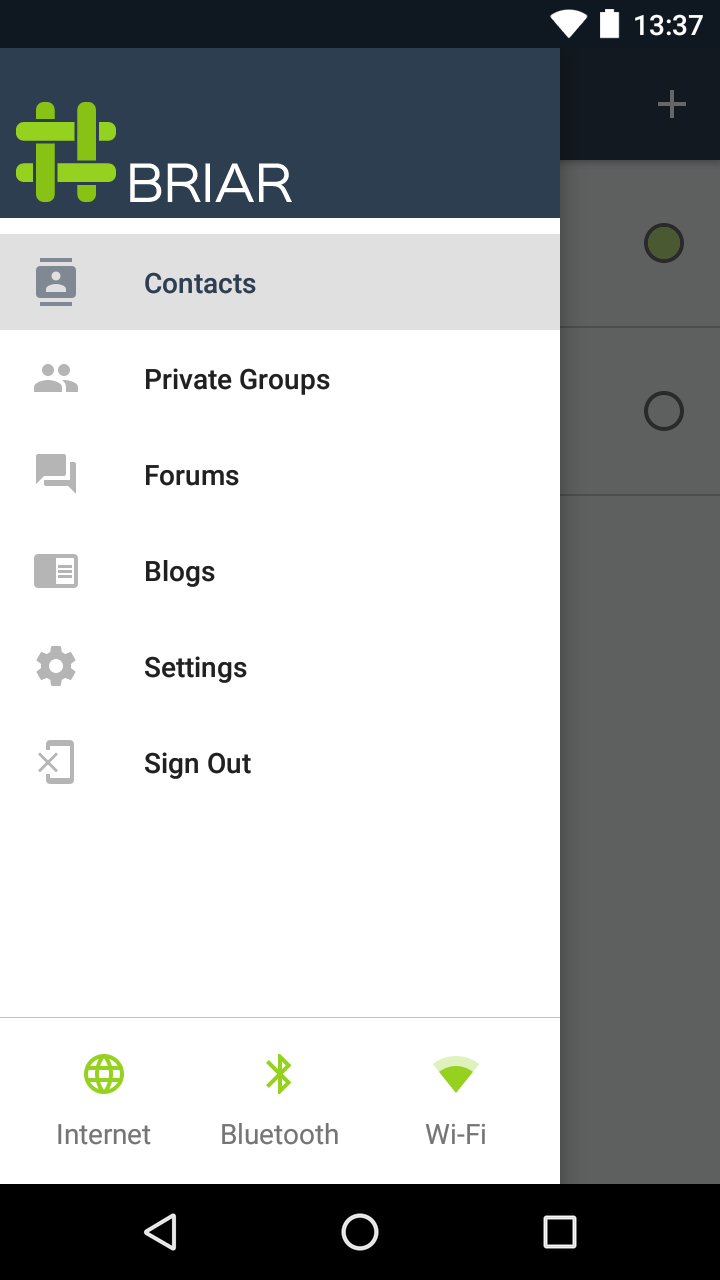
\includegraphics[width=0.2\textwidth]{briar1}
  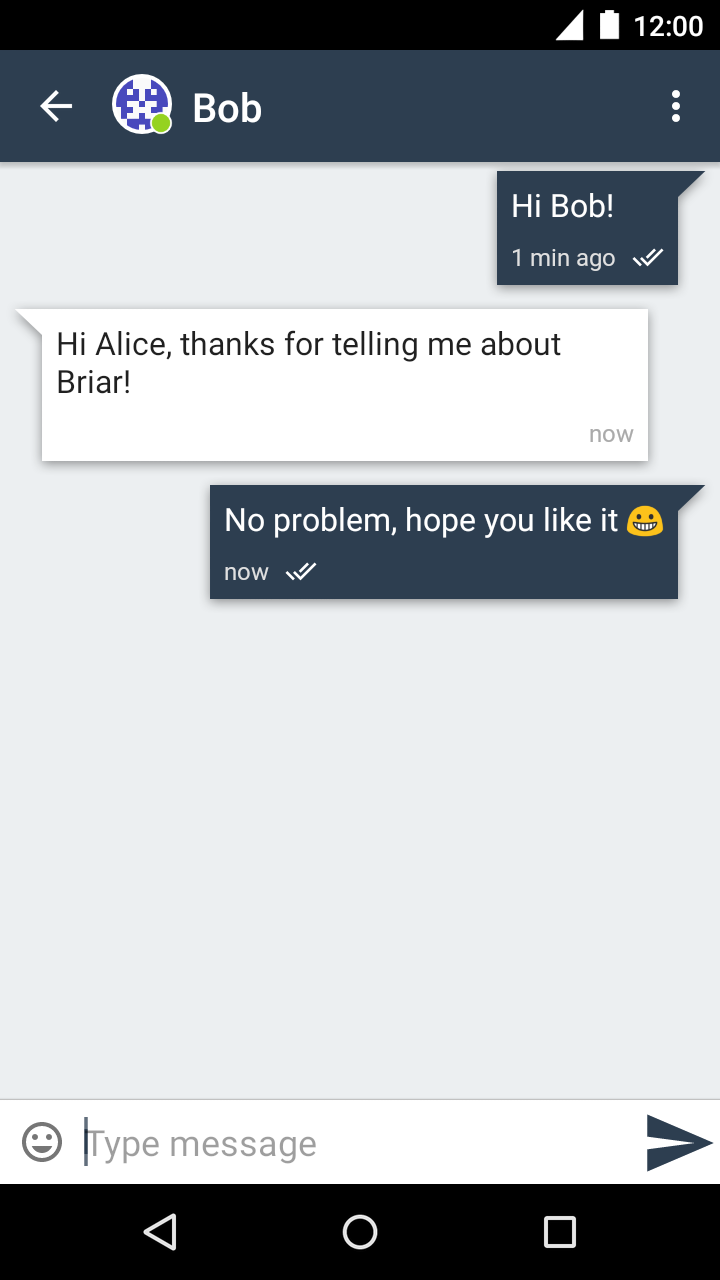
\includegraphics[width=0.2\textwidth]{briar2}
  \caption{The menu and conversation detail in Briar \cite{briar_gplay}}
\end{figure}

Briar \cite{briar_gplay} is an open-source project that started to support freedom of expression and right to privacy. It enables peer-to-peer encrypted messaging and forums. It is presented as a tool for activists, journalists, and anyone who needs a safe way to communicate.

Before the communication starts, users have to meet in person and scan QR codes from each other's screen. The devices exchange public keys and agree on a shared key using \textit{Bramble QR Code Protocol (BQP)} \cite{briar_bqp}.
%The protocol requires both devices to have Bluetooth enabled and be discoverable, or be connected to the same WiFi network.
This provides strong identities secure against man-in-the-middle attacks.

The device only accepts connections from devices in contacts. However, the user can initiate an introduction between two of her contacts. If both contacts accept the introduction request, then they are able to establish connections without meeting in person.

The communication is built on top \textit{Bramble Transport Protocol (BTP)} and \textit{Bramble Synchronization Protocol (BSP)}, transport and application layer protocols suitable for \textit{delay-tolerant networks}. \cite{briar_stack} It does not rely on any central server, but instead allows to synchronize messages using Bluetooth or Wi-Fi. If the Internet is available, it can also connect via the Tor network.

However, the application does not take advantage of mesh networking. It can only communicate with devices it is directly connected to.

\subsection{Bridgefy}

\begin{figure}[h]
  \centering
  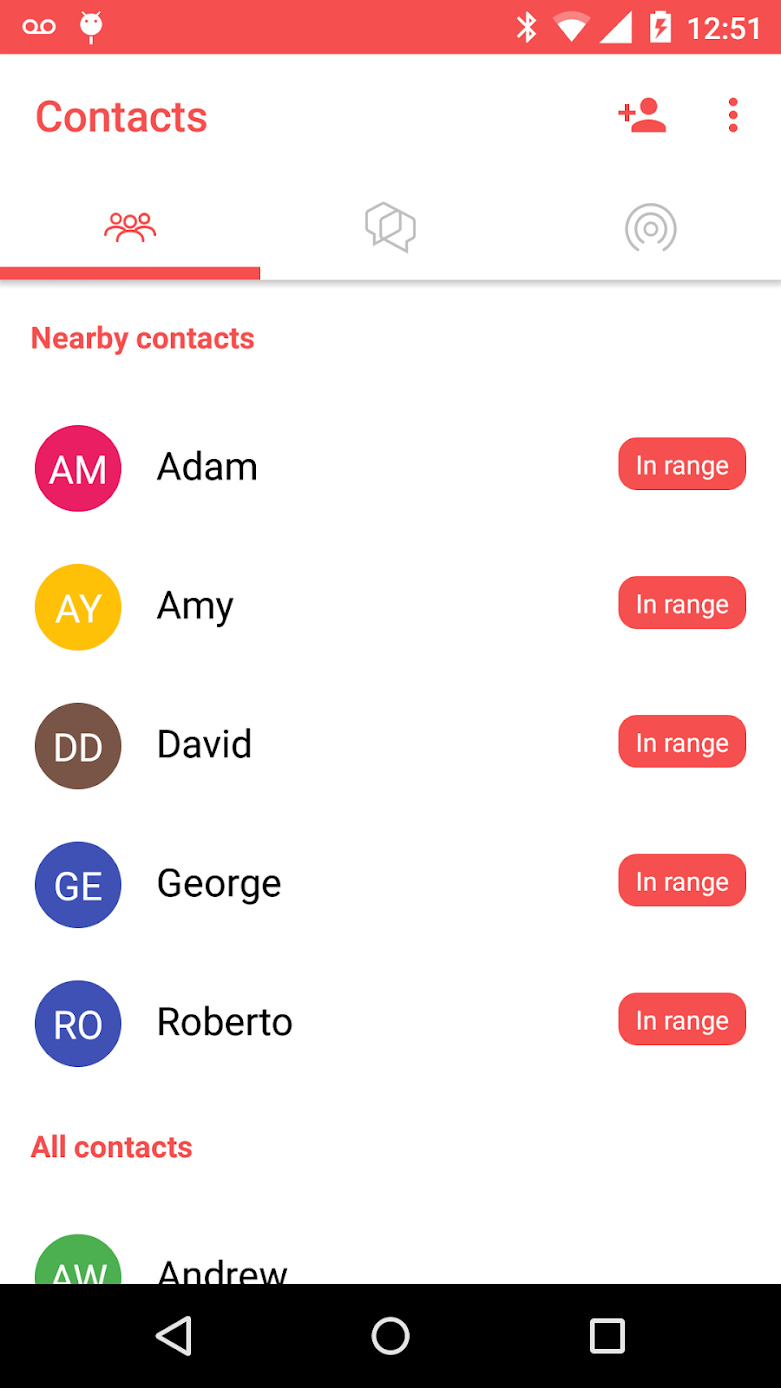
\includegraphics[width=0.2\textwidth]{bridgefy1}
  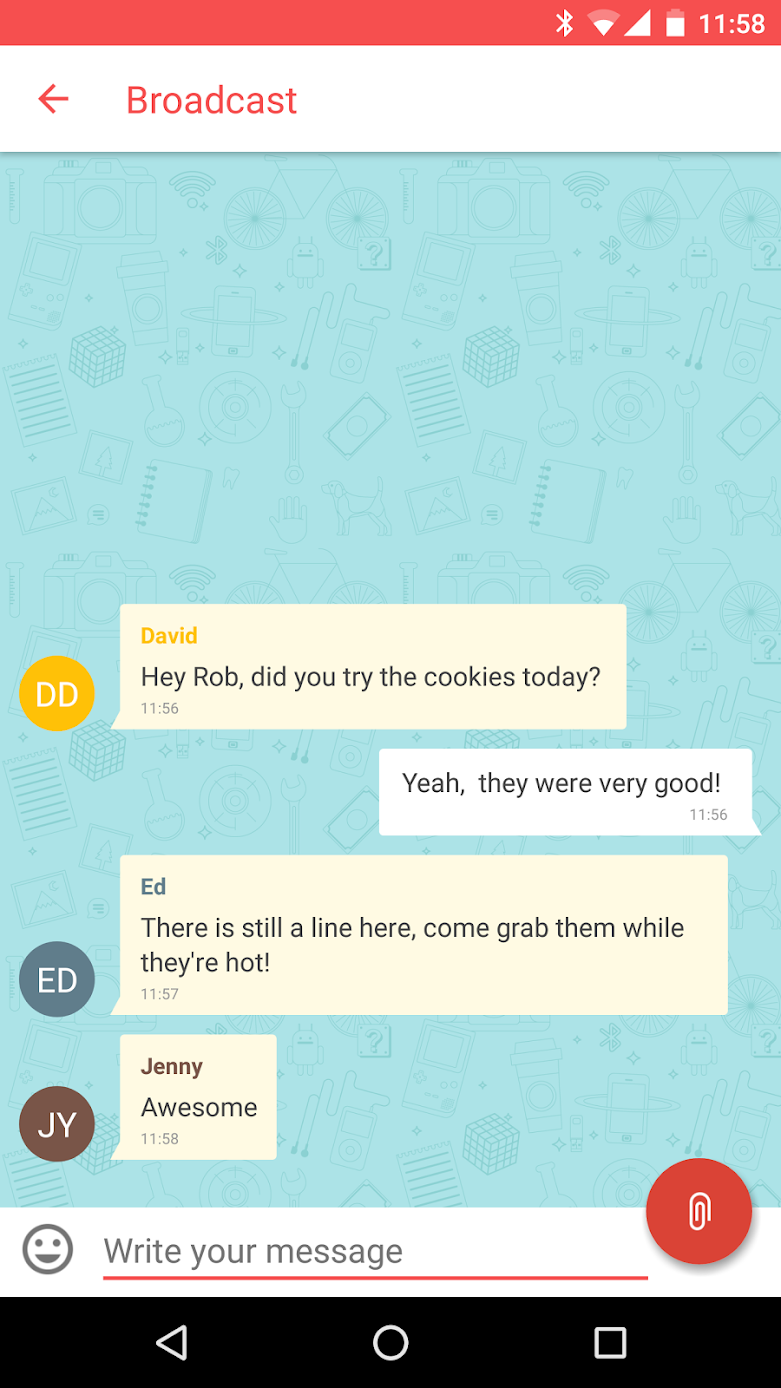
\includegraphics[width=0.2\textwidth]{bridgefy2}
  \caption{The list of nearby contacts and broadcasting in Bridgefy \cite{bridgefy_gplay}}
\end{figure}

Bridgefy is an offline messaging app based on Bluetooth connection. It can operate in 4 modes. Person to person mode allows to chat privately with users nearby. A mesh mode allows to route traffic through devices of other users using the app. The broadcast mode allows to broadcast and see messages of all people around, even those not in the contacts. Finally, the online mode allows to send messages anywhere in the world, provided the internet connection is available.

The app is built on top of Bridgefy SDK, a multi-platform SDK for building mesh networking apps. Both SDK and the app are proprietary. The SDK allows to send a point-to-point message to a specific device addressed by its ID, or to broadcast a message to all devices present in the mesh network.

The app requires the user to set up an account and perform a phone number verification. The SDK requires internet connection to verify the license. Finally, it requires a permission to access the contacts list. Therefore, while the app has gained popularity during the 2019 Hong Kong protests \cite{forbes:hk}, it does not work fully offline and raises some privacy concerns.

\subsection{FireChat}

\begin{figure}[h]
  \centering
  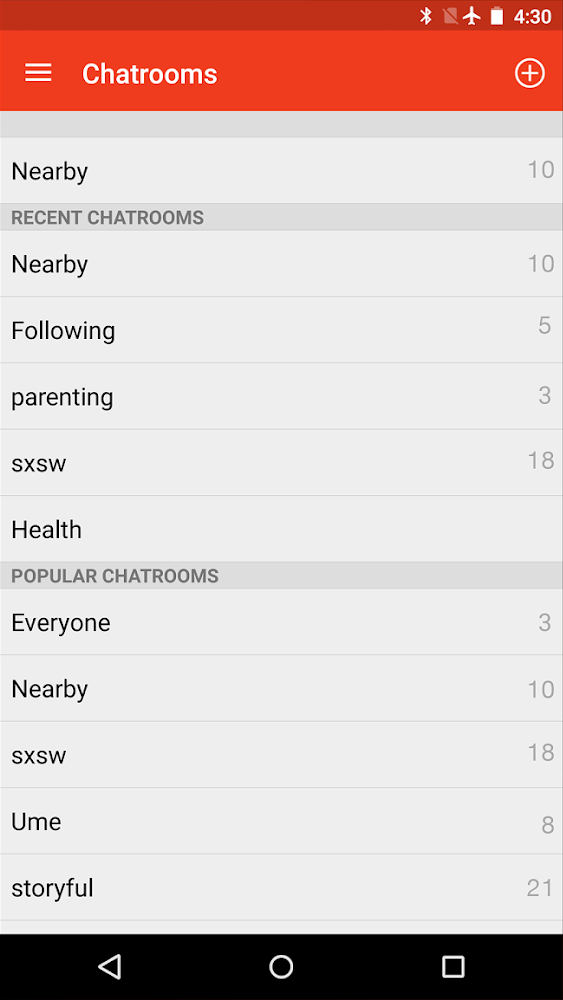
\includegraphics[width=0.2\textwidth]{firechat1}
  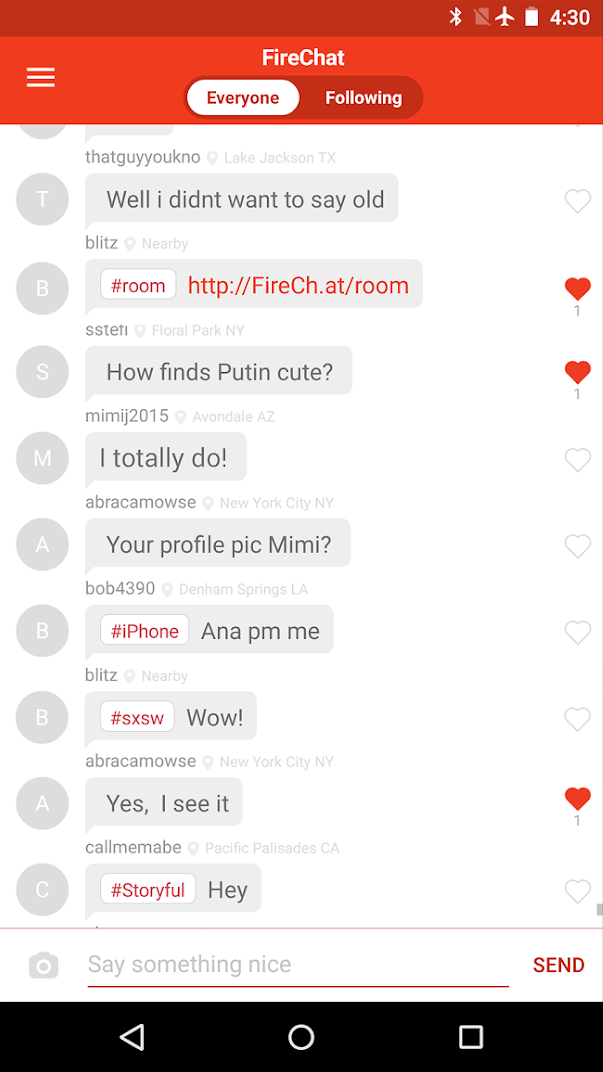
\includegraphics[width=0.2\textwidth]{firechat2}
  \caption{The list of rooms and a conversation detail in FireChat \cite{firechat}}
\end{figure}

FireChat \cite{firechat} is a proprietary offline messaging app built by OpenGarden. It uses Bluetooth and Wi-Fi to communicate with other devices, and takes advantage of multi-hop technology. It allows to send messages and photos, private messages with end-to-end encryption, create private groups, and use hashtags to create public chat rooms.

Similarly to Bridgefy, it requires internet connection for setting up an account. Unfortunately, we were not able to fully test the app at the time of writing this survey due to a bug in the sign up process.

\subsection{The Serval Mesh}

\begin{figure}[h]
  \centering
  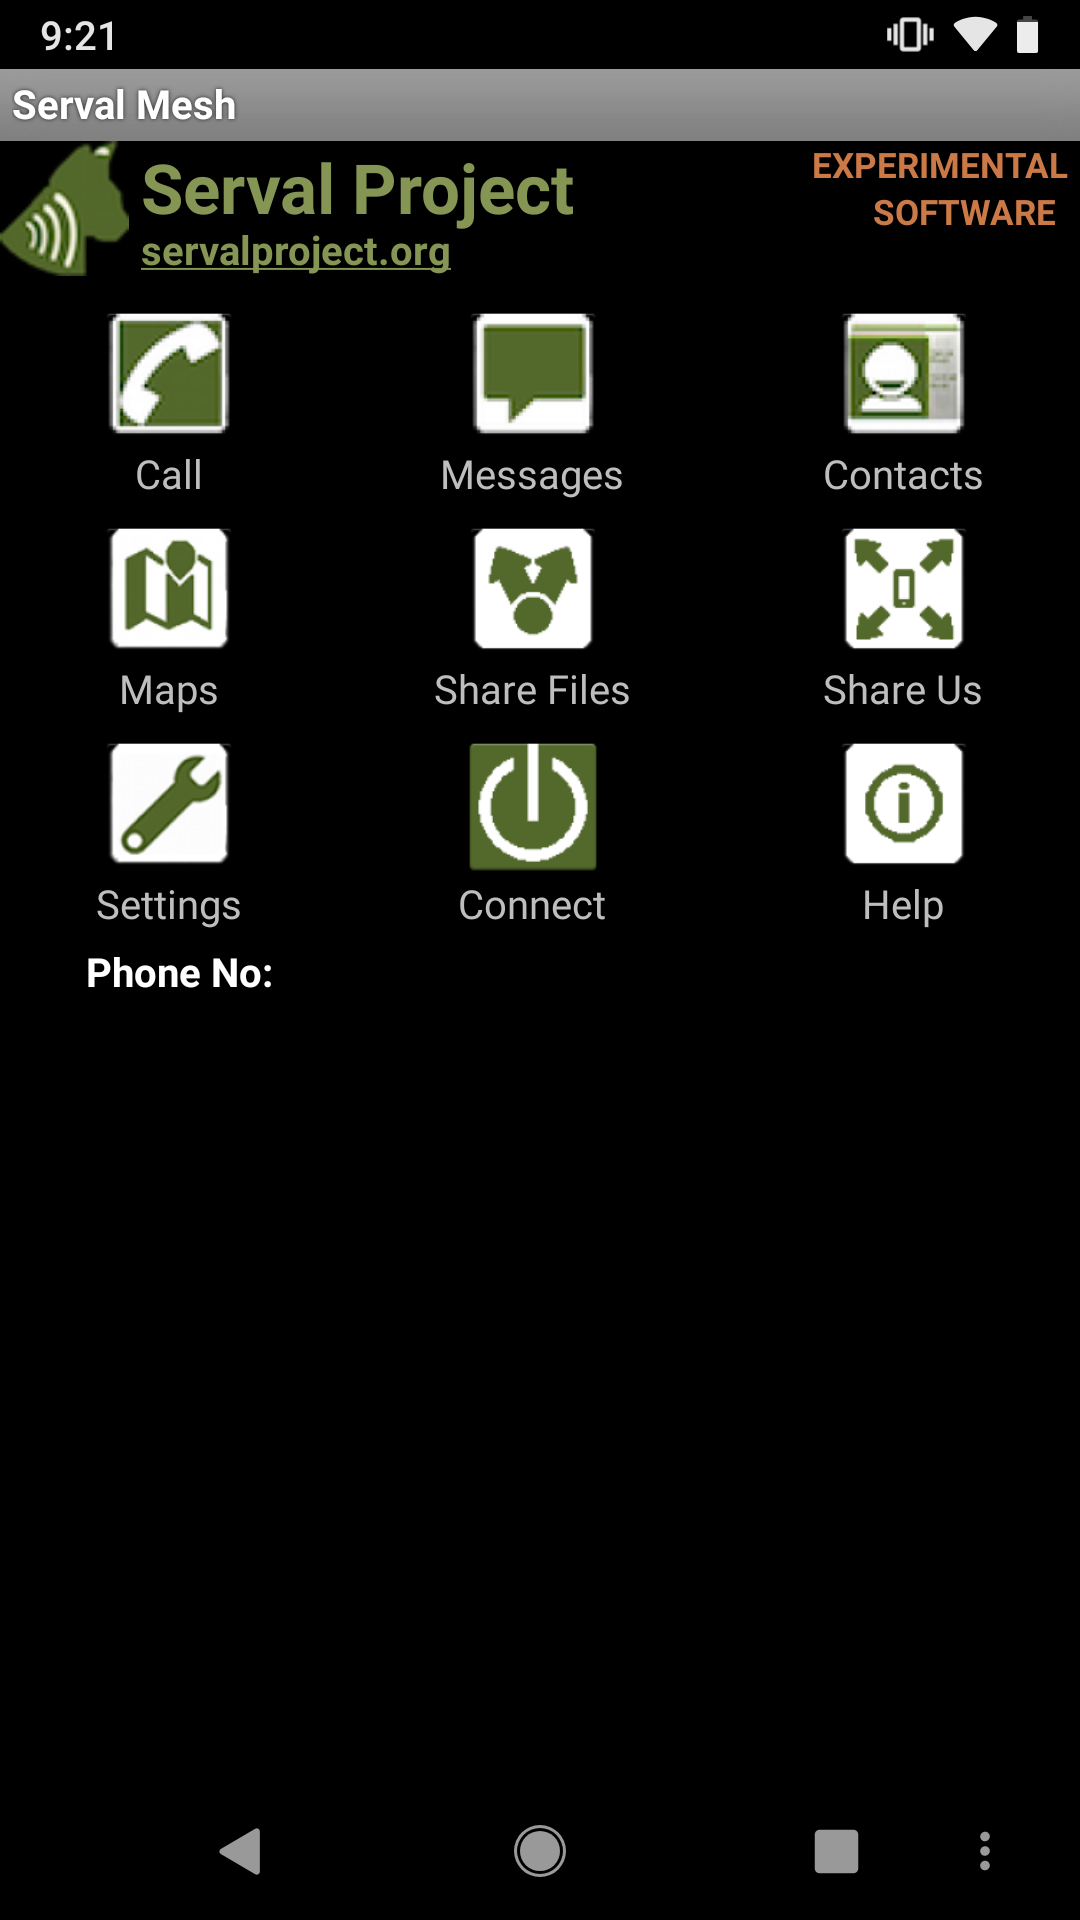
\includegraphics[width=0.2\textwidth]{serval1} 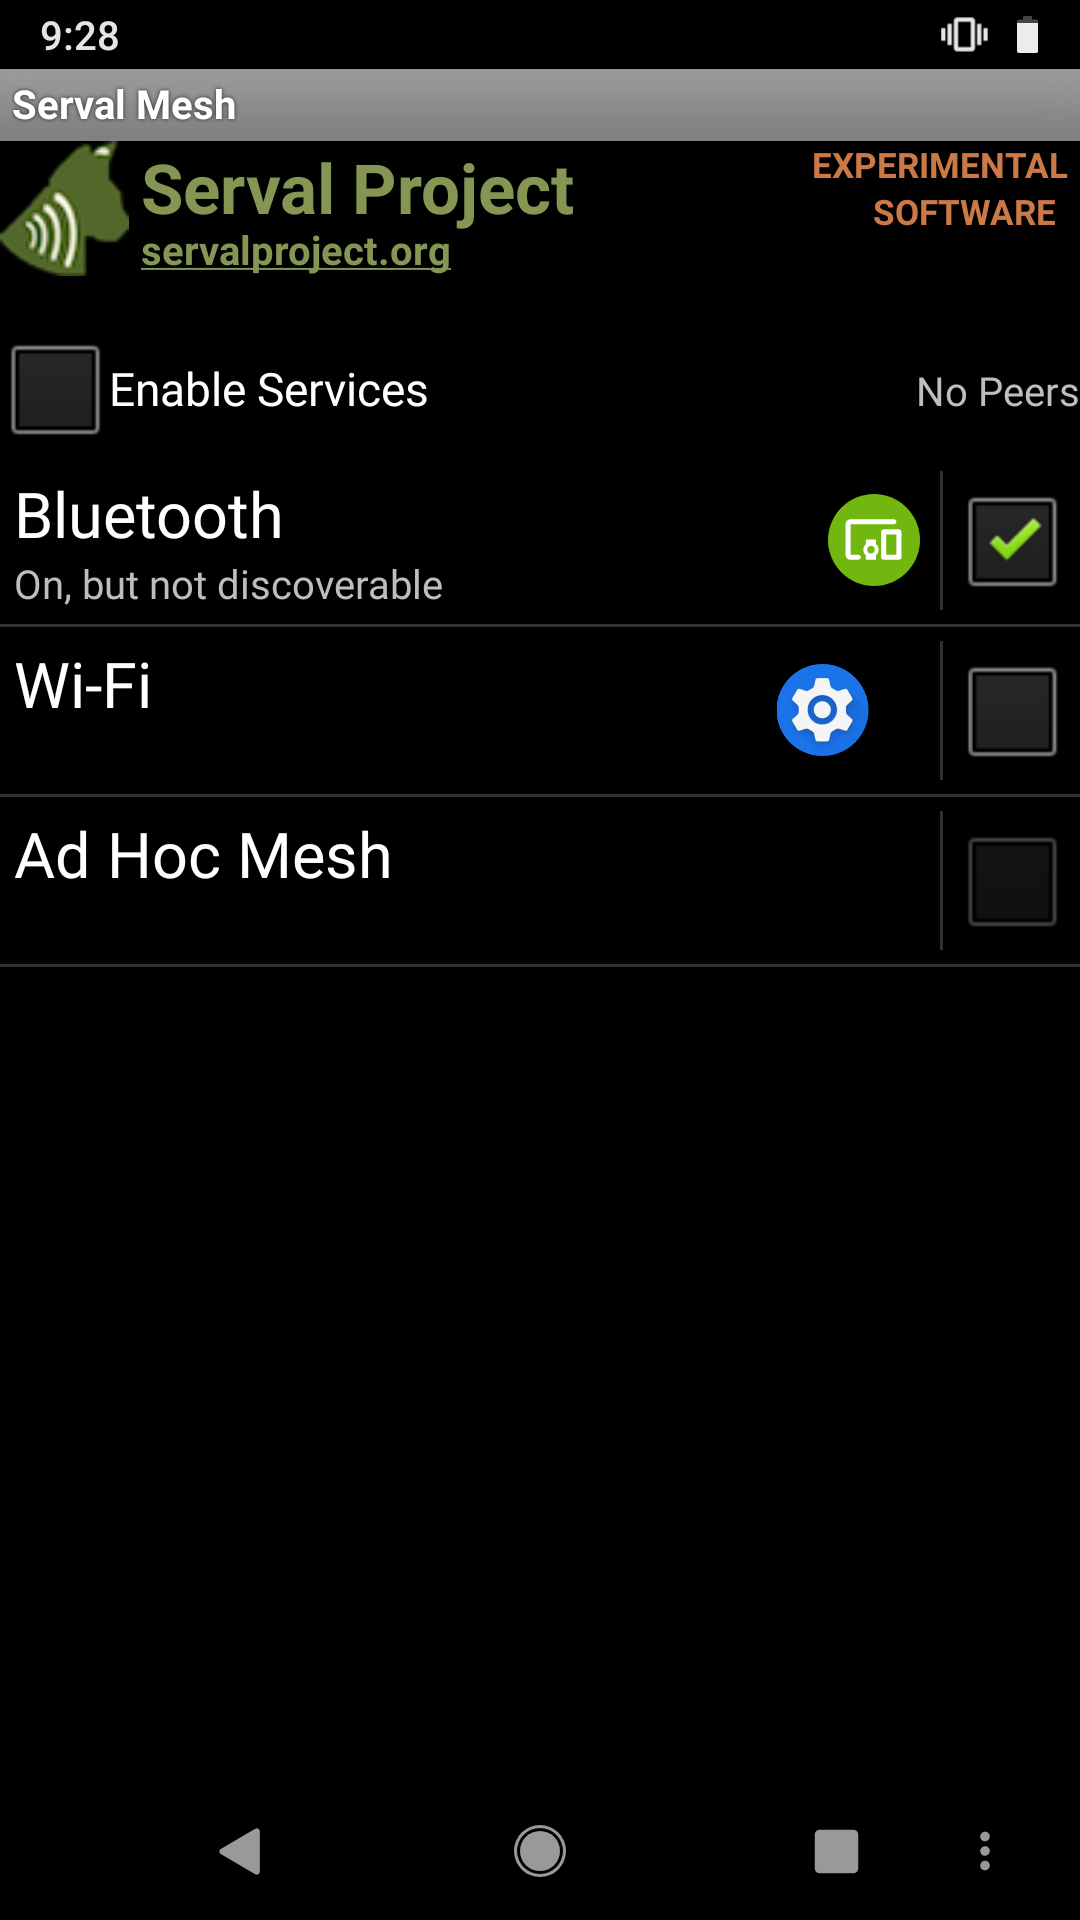
\includegraphics[width=0.2\textwidth]{serval2}
  \caption{The dashboard and connection settings in the Serval Mesh}
\end{figure}

The Serval Mesh \cite{serval} is an Android app that enables people to make voice calls, send text messages and even share files using without requiring any inftrustructure. networking. Its primary motivation is to provide resilient communication during crisis or disaster situations. It primarily uses Bluetooth and Wi-Fi. On supported devices, it can enable a Wi-Fi ad hoc mode when given a root access.

The Android application codenamed Batphone is based on \textit{Serval Distributed Numering Architecture} (DNA) \cite{servaldna}, the core daemon implementing services in the mesh network. Each device in the network is identified by its phone number, which the user can claim. To call a number, the app broadcasts \texttt{DNA LOOKUP} request to nearby devices. The \textit{Mesh Datagram Protocol} (MDP) is a broadcast mechanism that propagates the request to all devices recursively, while respecting TTL. Any device receving a the request sends \texttt{DNA REPLY} response. The originating device collects all responses and shows the list to the user. As any user can claim any phone number, this mechanism is vulnerable to impersonation if the user claims a number they do not own.

Voice calls are implemented by \textit{Voice over Mesh Protocol} (VoMP), a custom two-way audio streaming protocol. It has been designed to work in unstable conditions of wireless mesh networks by allowing mid-call re-routing and re-connection.

\textit{Rhizome} is a content distribution service with a content-exchange protocol based of MDP. Each piece of content is called a \textit{bundle}. The bundle consists of a \textit{manifest} describing its content, and a \textit{payload}. \textit{MeshMS} is then a service implemented on top of Rhizome that allows sending short text messages.

The latest version has been released in 2016 and it does not seem to be in active development. It is also incompatible with recent versions of Android and requires root for mesh functionality.

\subsection{Hype SDK}
The Hype SDK \cite{hype} is a cross-platform mesh networking library. It is based on the \textit{multi-transport} concept, where multiple communication technologies can be used simulateneously. Currently, Hype supports Wi-Fi Infrastructure, Wi-Fi Direct, Bluetooth Classic, and Bluetooth Low Energy. The developer is given choice which transports to enable based on the badwidth or power efficiency requirements of the application.

When a new node is found, a \textit{found notification} is triggered. The notification includes a device id and an optional user id. If the app decides to establish a connection with the discovered node, it requests a handshake. This process is also referred to as \textit{resolving an instance}. During the handshake, devices exchange public encryption keys, announcements, and other connection configurations.

The Hype SDK also enables remote connectivity by integrating the concept of \textit{Internet reachability}. A Hype-enabled device can connect with other peers over the Internet, using NAT traversal techniques or a central server operated by Hype Labs.

All communication is end-to-end encrypted to ensure confidentiality and integrity of transferred messages. To provide authenticity, each device is issued a certificate by a central server before joining the network. For that reason, the device needs to be connected to the Internet when joining the network for the first time, or when the certificate expires.

The Hype SDK is offered as a paid service with billing based on the number of monthly active devices.

In mesh networks, nodes are required to cooperate by forwarding content on behalf of each other. With Internet reachability enabled, this also means sending packets over the Internet, which can be a scarce resource. HypeLabs is currently working on the implementation of \textit{Hype Open Protocol} (HOP), which aims to incentivize nodes to remain active in the network. HOP will likely take advantage of a utility token based on the \textit{Stellar Consensus Protocol}. Consequently, a fee can be charged by nodes for routing traffic or providing Internet connectivity. It is still in an early development stage with a public release planned for 2021. \cite{hop}

%\subsection{p2pkit}

\subsection{Nearby Connections API}

All previously mentioned technologies can be accessed on Android directly using their corresponding APIs. However, in some cases, the behavior depends on the version of Android OS or even device-specific implementation. Moreover, every API is slightly different, and taking advantage of multiple technologies simultaneously takes considerable effort. For that reason, Google introduced Nearby Connections API in 2015 and its fully-offline version 2.0 in 2018. \cite{nearby2} The API aims to large extent simplify development of Android applications relying on peer to peer communication. It is able to automatically switch between Bluetooth, BLE, Wi-Fi, Wi-Fi Direct, and Wi-Fi Aware depending on the application needs and device capabilities.

It supports multiple strategies for different network topologies, specifically cluster, star, and point to point. The cluster topology is the most general one allowing m-to-n connections. However, in the current version, the cluster stratgy results in lower bandwidth connections as it uses only Bluetooth connectivity.

The library is closed-sourced, but it has been previously reverse-engineered and analyzed by security researchers. Several vulnerabilities have been discovered and disclosed to Google, including impersonation, man-in-the-middle attacks, attacker-induced physical layer switch, DoS, or radio state manipulation. \cite{nearbytr}

The library is distributed as part of Google Play Services, which means it is only available on devices that are certified by Google. This also prevents it from being used in countries where access to Google is restricted. This is not compatible with our idea of censorship resilient communication.


\section{Our Proof of Concept} \label{poc}

\begin{figure}[h]
  \centering
  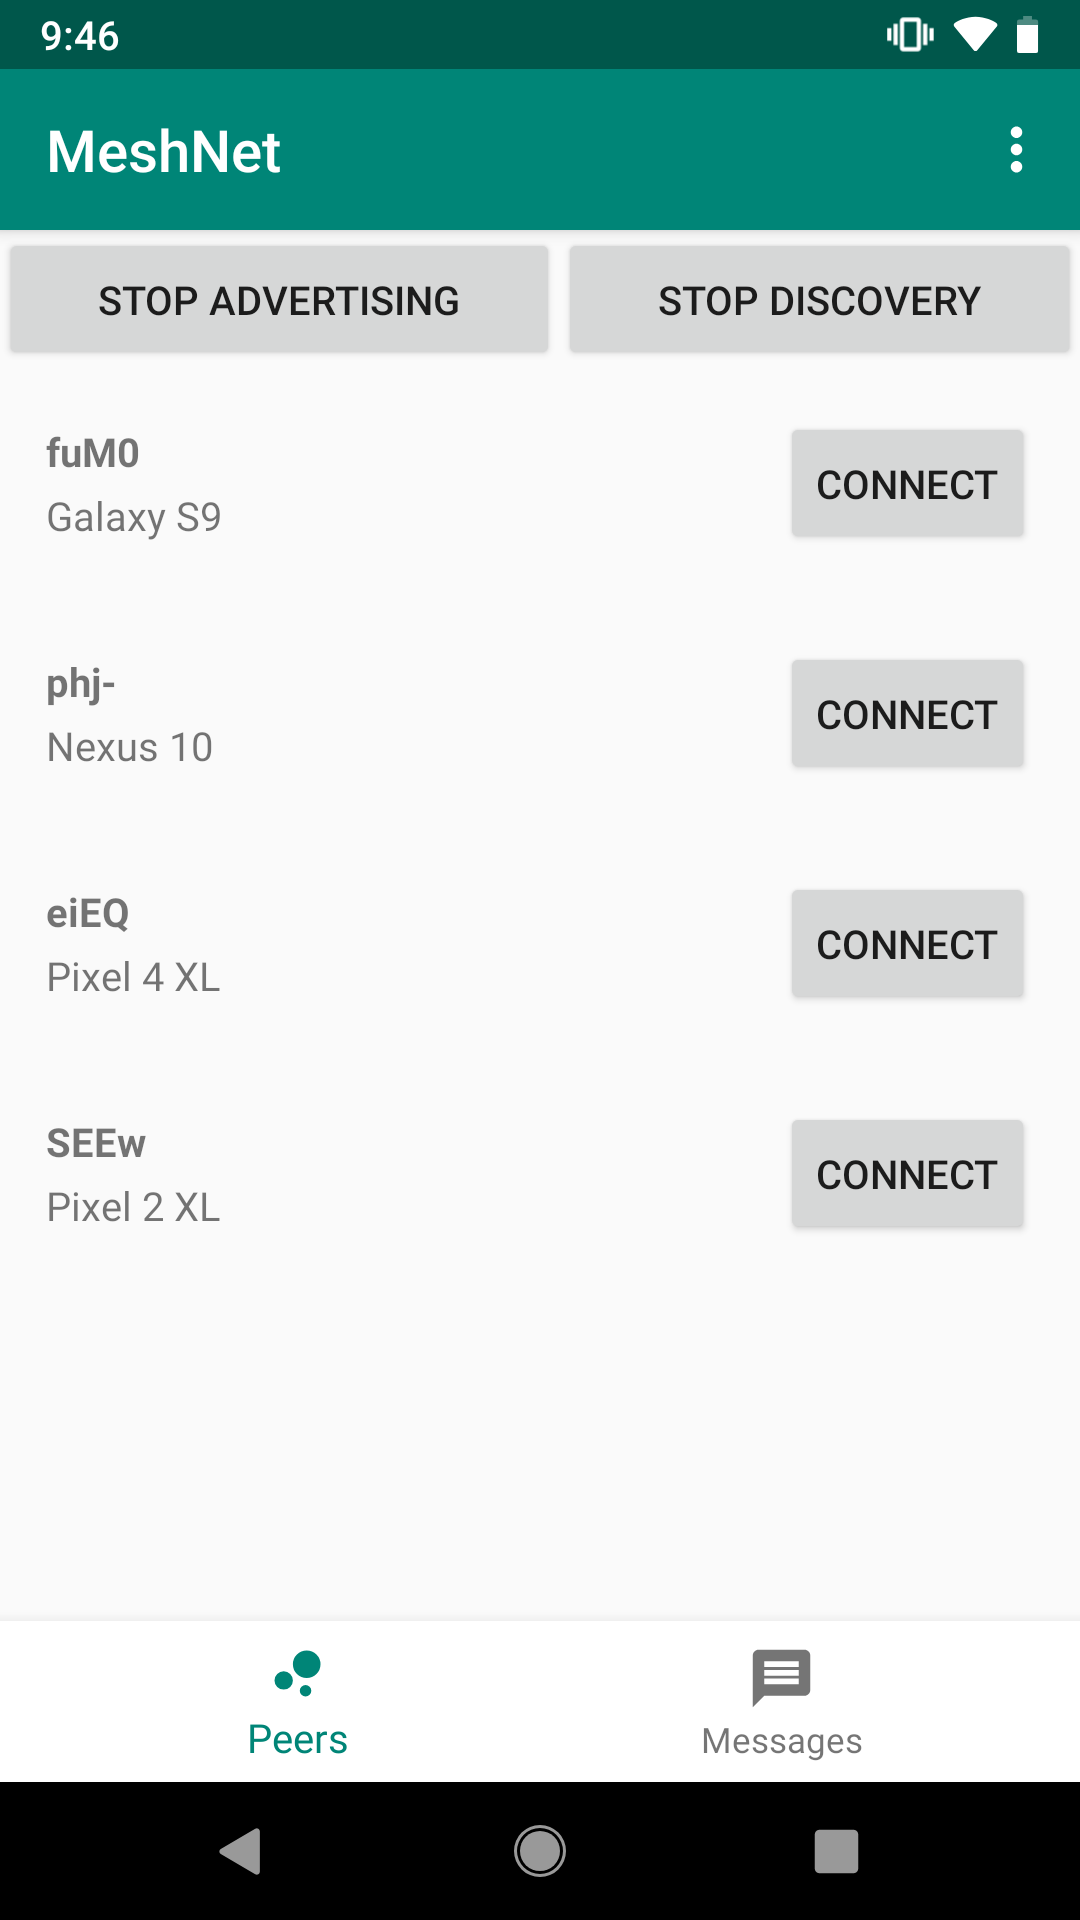
\includegraphics[width=0.2\textwidth]{meshnet1} 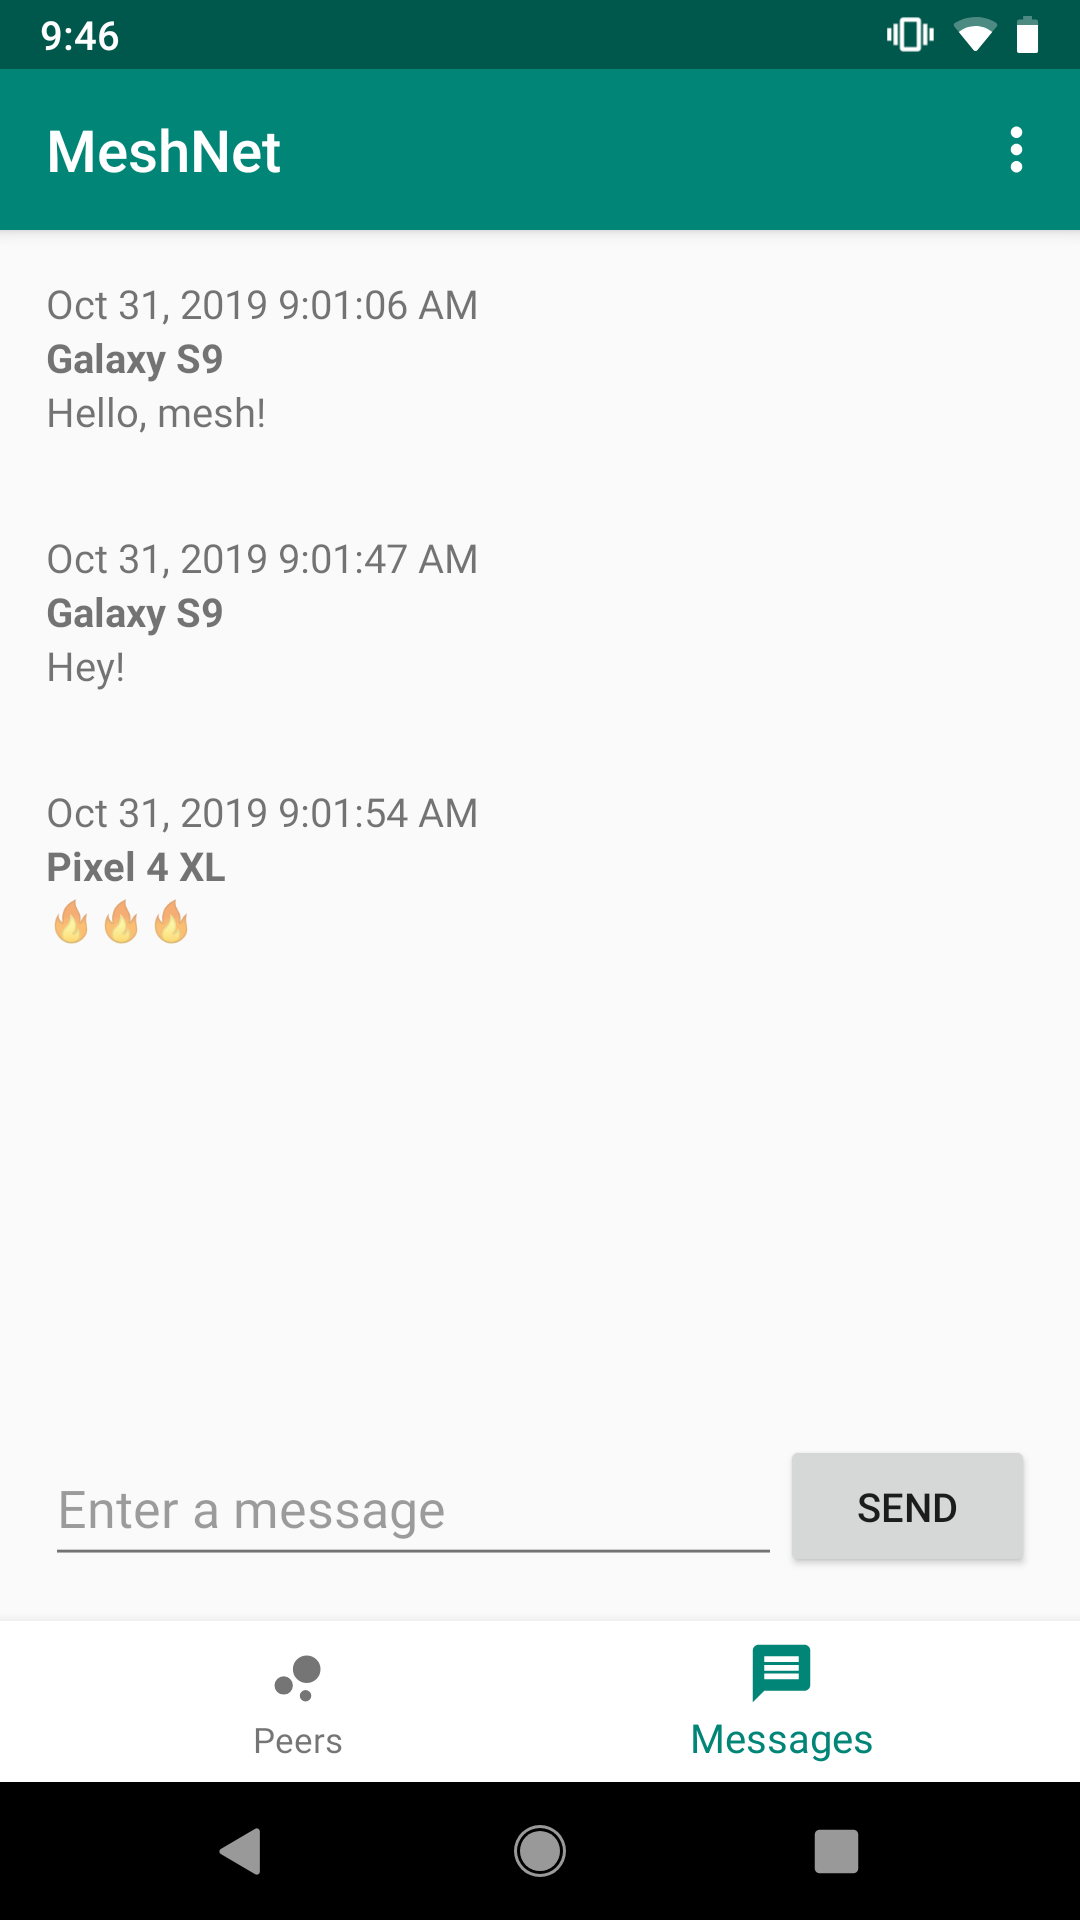
\includegraphics[width=0.2\textwidth]{meshnet2}
  \caption{Our proof of concept MeshNet app}
\end{figure}


To explore various wireless communication capabilities of current smartphone devices, we have developed a simple demo application MeshNet. First, we have defined a common connectivity interface, and then made several implementations using all connectivity APIs currently available on Android. It is possible to choose the transport layer from Bluetooth, Bluetooth with BLE discovery, BLE GATT, BLE L2CAP, Wi-Fi Direct, Wi-Fi Aware, and Nearby Connections API.

Secondly, we have implemented a rudimentary mesh network using store and forward principle based on flooding. Once the app receives a message, it first checks if it has not been received before to prevent loops. Then it stores it and forwards it to all other peers.

The source code of the resulting application is publicly available\footnote{https://github.com/MattSkala/meshnet-android}. Aside from being a functional prototype, it can also serve as a reference for implementing connectivity APIs on Android, as we noticed that the official documentation is often incomplete and occasionally contains mistakes.

% simple, but more complicated comunication protocols feasible

\section{Conclusion} \label{conclusion}

% required internet connection/not working with the latest android/not providing mesh networking

In this survey, we have first introduced several wireless communication technologies. Then, we have analyzed state-of-the-art SDKs and applications taking advantage of those technologies to provide offline communication. We have seen that up to date, there is no censorship-resilient communication app that would be able to work without any infrastructure, be secure, and compatible with the majority of recent devices. Most of the apps available today still require internet connection at least for initial setup, or are susceptible to man-in-the-middle attacks. Last but not least, most of them are proprietary solutions based on a closed source code, relying on security by obscurity.
To that end, we have shown that it is feasible with technologies available today to build a fully offline mesh networking solution using several wireless technologies.

As future work, we envision an open-source universal communication protocol that would be able to take advantage of communication technologies available to a given device. The protocol should allow to build a hybrid network by routing traffic between devices in a mesh network and the Internet. The protocol should have NAT puncturing built-in to be able to facilitate direct connections between devices over the Internet without need for any central server. Finally, there should be a way to incentivize routing of traffic in the network to prevent DoS attacks. To our best knowledge, this has not been achieved yet and still poses some open research questions.

\bibliographystyle{IEEEtran}
\bibliography{mybibfile}

\end{document}
